\chapter{Phase Space Integration}
If an unstable particle of mass $m_A$ decays to $N$ particles with four momenta $p_1,p_2...p_N\equiv\{p_f\}$
the differential decay rate is
\begin{equation}
d\Gamma = \frac{1}{2m_A}|\mathcal{M}(m_A\rightarrow\{p_f\})|^2d\Phi_{\text{lips}}(p_A\rightarrow\{p_f\})
\end{equation}
where the Lorentz-invariant phase space is defined as
\begin{equation}
d\Phi_{\text{lips}}(p_A\rightarrow\{p_f\}) \equiv \left(\prod_f\frac{d^3p_f}{(2\pi)^3}\frac{1}{2E_f}\right)(2\pi)^4\delta^{(4)}\left(p_A-\sum_i p_i\right).
\end{equation}
\paragraph{Two particle final-state}
In the case of only two final-state-particles with three momentum $\pm \vec{p}$ the phase space can be written as
\begin{equation}
d\Phi_{\text{lips}}(p_A\rightarrow\{p_1,p_2\})=\int \frac{\Omega_{\text{cm}}}{4\pi} \frac{1}{8\pi}\left(\frac{2|\vec{p}|}{E_\text{cm}}\right) 
\end{equation}
\paragraph{Three particle final-state}
The three particle case can still be solved relatively strait forward with some algebra and kinematical considerations. Though there is a ready to use recipe by Asatrian
\cite{Asatrian:2012tp}. Here one starts with "dimensionless" momenta $p'_i=p_i/m_A$ and works in the rest frame of $p_1$ and $p_3$ where $q' = p'_1+p'_2=(\sqrt{s_{13}},\vec{0})^T$.
The coordinate system can then be rotated such that the remaining two momenta are given by
\begin{align}
p'&=(E',|\vec{p'}|,0,0)\\
p'_3&=(E'_3,|\vec{p'_3}|\cos\theta,|\vec{p'_3}|\sin \theta,0).
\end{align}
With the mass fractions $x_i = m_i^2/m_A^2$ this may be expressed with
\begin{align*}
|\vec{p'}| &= \frac{1}{2\sqrt{s_{13}}}\sqrt{(1+x_2-s_{13})^2-4x_2}\\
|\vec{p'_3}|&=\frac{1}{2\sqrt{s_{13}}}\sqrt{(x_1+x_3-s_{13})^2-4x_1x_3}
\end{align*}
With
\begin{equation}
X\equiv -4|\vec{p'}||\vec{p'_3}|\cos\theta+1+2(x_1+x_3)-s_{13}-\frac{(1+s_{13}-x_2)(x_1-x_3)}{s_{13}}
\end{equation}
this can be used to express all combinations of momenta in scalar products in the matrix element by the following combinations:
\begin{align}
p'_i\cdot p'_i&= x_i\\
p'\cdot p'_1&=\frac{2(1+x_1+x_3)-x_2-X}{4}\\
p'\cdot p'_2&=\frac{1+x_2-s_{13}}{2}\\
p'\cdot p'_3&=\frac{-2(x_1+x_3)-x_2+2s_{13}+X}{4}\\
p'_1\cdot p'_2&=\frac{2+4x_3-x_2-2s_{13}-X}{4}\\
p'_1\cdot p'_3&=\frac{s_{13}-x_1-x_3}{2}\\
p'_2\cdot p'_3&= \frac{-x_2-4x_3+X}{4}.
\end{align}
The phase space integral can then be written as
\begin{equation}
d\Phi_{\text{lips}}(p_A\rightarrow\{p_1,p_2,p_3\})=\frac{m_A^2}{8(2\pi )^3}|\vec{p'}||\vec{p'_3}|d\cos\theta d s_{13}
\end{equation}
where $\cos\theta$ is to be integrated from $-1$ to $1$ and $s_{13}$ from $(\sqrt{x_1}+\sqrt{x_3})^2$ to $(1-\sqrt{x_2})^2$.
\paragraph{Four particle final-state for a polarised decay}
All in all there will be seven independent variables of integration. Asatrian gives also a recipe for this case. However, for this work, the differential decay rate of the decay in four particles is needed and Asatrian's method doesn't permit that.
Since there is virtually no hope in finding an analytical solution to all integrals encountered in this task, one might as well start in a direction that does allow relatively strait forward evaluation with numerical methods. 
To simplify matters lets work in the rest-frame of the decaying particle, adopt spherical coordinates $dp^3 \equiv d|p|d\Omega$ and specialise in the case, where particle three is massless.
Firstly, one may eliminate the overall energy-momentum conserving four delta distributions by replacing the three $p_4$ integrals using (writing the time component of $p_4$ as $E_4$ even though its not on shell)
\begin{equation}
\int\frac{d^3p_4}{2E_4}=\int d^4p_4\delta(p_4^2-m_4^2)\Theta(E_4)
\label{eq:AppOffShell}
\end{equation}
and carrying out the $dp_4$ integral:
\begin{align*}
\frac{1}{(2\pi)^8} \frac{d^3p_1}{2E_1}\frac{d^3p_2}{2E_2}\frac{d^3p_3}{2E_3}\delta\left((p_A-\sum_{i=1}^3p_i)^2-m_4^2\right)\Theta(m_A-\sum_{i=1}^3E_i)
\end{align*}
and changing the momenta to the energies
\begin{align*}
\frac{1}{2^3(2\pi)^8}\sqrt{E_1^2-m_1^2}\sqrt{E_2^2-m_2^2}E_3dE_1dE_2dE_3d\Omega_1d\Omega_2d\Omega_3\times \\ \delta\left((p_A-\sum_{i=1}^3p_i)^2-m_4^2\right)\Theta(m_A-\sum_{i=1}^3E_i).
\end{align*}
At this point it is advisable to adopt a specific coordinate frame where the z-axis is already fixed by the spin of the decaying particle:
\begin{align}
p_A&=(m_A,0,0,0)\\
p_1&=(E_1,\sqrt{E_1^2-m_1^2}\sin\theta_1,0,\sqrt{E_1^2-m_1^2}\cos\theta_1)\\
p_2&=(E_2,\sqrt{E_2^2-m_2^2}\sin\theta_2\cos\phi_2,\sqrt{E_2^2-m_2^2}\sin\theta_2\sin\phi_2,\sqrt{E_2^2-m_2^2}\cos\theta_2)\\
p_3&=(E_3,E_3\sin\theta_3\cos\phi_3,E_3\sin\theta_3\sin\phi_3,E_3^2\cos\theta_3)
\label{eq:momenta}
\end{align}
Now the phase-space weight and any momentum-scalar products are independent of $\phi_1$ so the integral can be carried out resulting in another factor of $2\pi$.

Lets now turn our attention to the delta distribution 
\begin{equation}
\int dE_3 \delta\left(\left(p_A-\sum_{i=1}^3p_i\right)^2-m_4^2\right)
\end{equation}
and use the $E_3$ integration to get rid of it:
\begin{align}
\begin{split}
=&\int dE_3 \delta(m_A^2+m_1^2+m_2^3-m_4^2-2m_A(E_1+E_2+E_3)\\
&-2E_1E_2+2\sqrt{E_1^2-m_1^2}\sqrt{E_2^2-m_2^2}(\sin\theta_1\sin\theta_2\cos\phi_2+\cos\theta_1\cos\theta_2))\\
&-2E_1E_3+2\sqrt{E_1^2-m_1^2}E_3(\sin\theta_1\sin\theta_3\cos\phi_3+\cos\theta_1\cos\theta_3))\\
&-2E_2E_3++2\sqrt{E_2^2-m_2^2}\sqrt{E_3^2-m_2^3}(\sin\theta_2\cos\phi_2\sin\theta_3\cos\phi_3\\
&+\sin\theta_2\sin\phi_2\sin\theta_3\sin\phi_3+\cos\theta_2\cos\theta_3))\\
=&\lvert-2\sqrt{E_1^2-m_1^2}(\sin\phi_3\sin\theta_1\sin\theta_3+\cos\theta_1\cos\theta_3)+2E_1-2\sqrt{E_2^2-m_2^2}\\&\cdot(\sin\theta_2\sin\theta_3\cos(\phi_2-\phi_3)+\cos\theta_2\cos\theta_3)+2E_2-2m_a\rvert^{-1}\theta(\widetilde{E}_3)\\
\equiv&|\alpha|\theta(\widetilde{E}_3)
\end{split}
\end{align}
with
\begin{align*}
\widetilde{E}_3=&\alpha\Bigl{(}2\sqrt{E_1^2-m_1^2}\sqrt{E_2^2-m_2^2}(\sin\phi_2\sin\theta_1\sin\theta_2+\cos\theta_1\cos\theta_2)\\&-2E_1E_2+2E_1m_A+2E_2m_A-m_A^2-m_1^2-m_2^2\Bigr{)}
\end{align*}
where the Heaviside function comes from using equation \ref{eq:AppOffShell} to carry out the integration off-shell to ensure that the argument of the delta distribution has a root on the integration interval.

\chapter{Additional Bounds on Chiral Couplings}
Here additional bounds on coupling to the leptons that depend on the chirality are presented. These can be introduced by terms like
\begin{align}
\mathcal{L} &\supset \sum_{l=e,\mu,\tau}g'_{l,L}\cdot\bar{L}_l\gamma_\mu A'^\mu L_l+\sum_{l=e,\mu,\tau}g'_{l,R}\cdot\bar{e}_{lR}\gamma_\mu A'^\mu e_{lR}\\
&=\sum_{l=e,\mu,\tau} g'_{l,L}\left(\bar{l}\gamma^\mu A'_\mu P_L l+\bar{\nu}_l\gamma^\mu A'_\mu \nu_l\right)+\sum_{l=e,\mu,\tau} g'_{l,R}\bar{l}\gamma^\mu A'_\mu P_R l
\end{align}
Competing bounds will not be explicitly stated, because these models are not treated separately in the literature, even though some may be extrapolated. 
\begin{figure}[H]
  \centering
    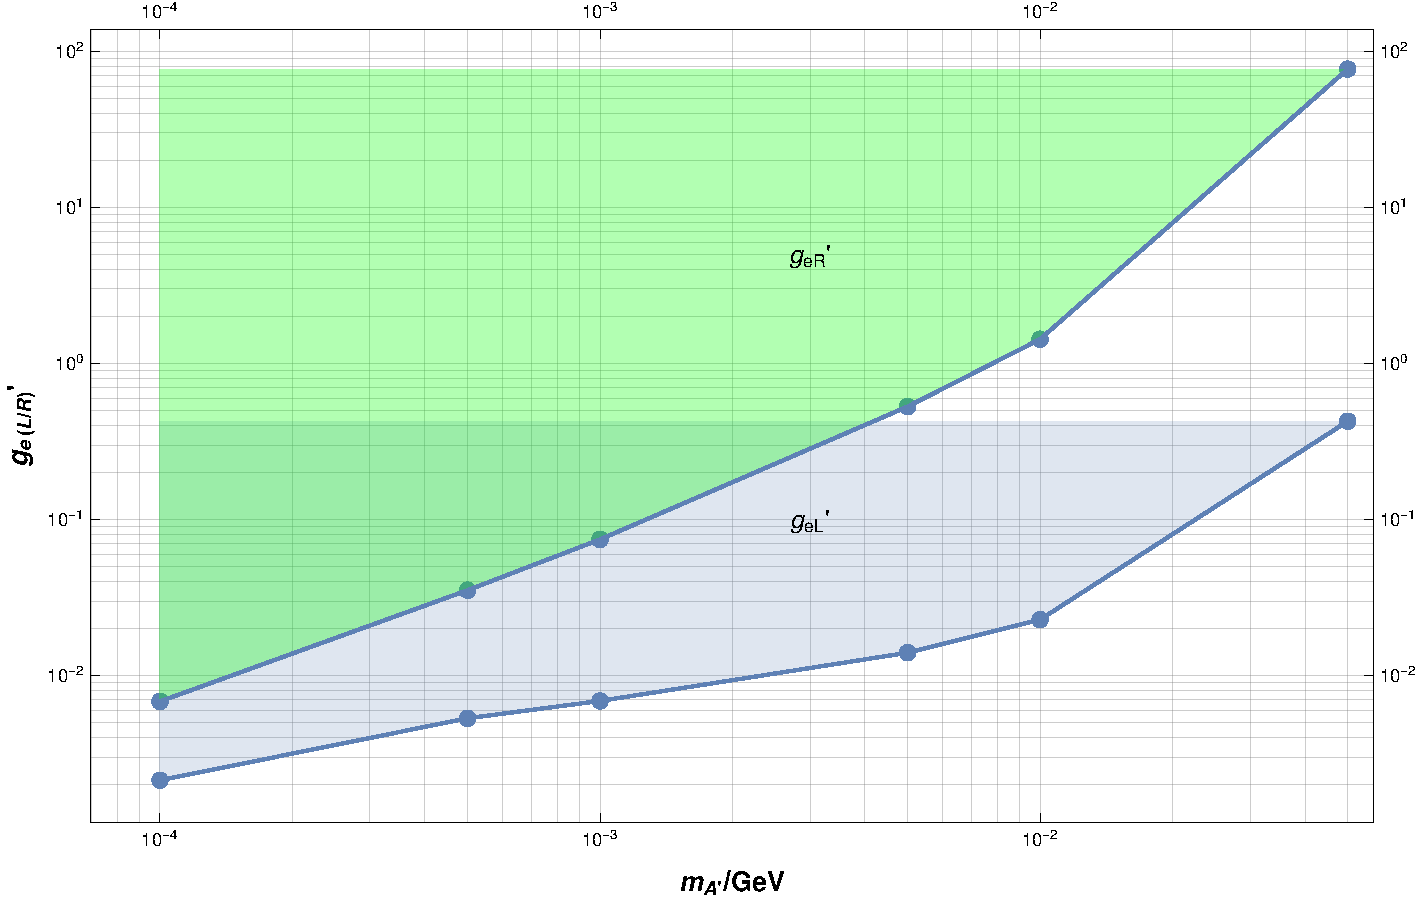
\includegraphics[width=\textwidth]{imgs/BoundERL}
    \caption{Bound on the left/right exclusive couplings to the electron}
    \label{fg:ERLBound}
\end{figure}
\begin{figure}[H]
  \centering
    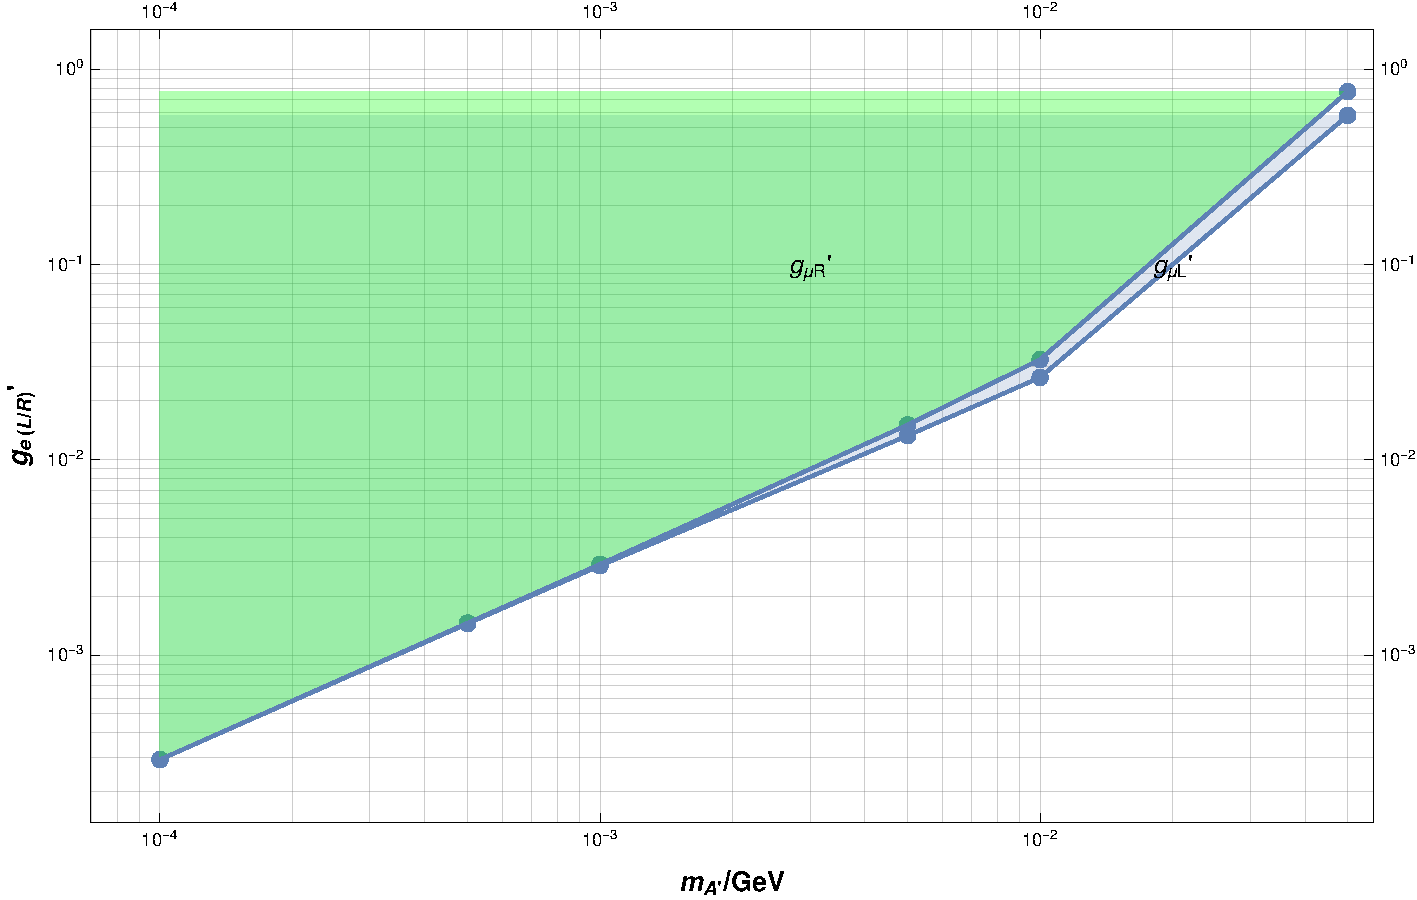
\includegraphics[width=\textwidth]{imgs/BoundMRL}
    \caption{Bound on the left/right exclusive couplings to the muon}
    \label{fg:MRLBound}
\end{figure}